\subsection{Baseline}

We are given that the policy gradient theorem can be generalized to include an arbitrary baseline $b(s)$:
\[
\nabla_\theta J(\pi) = \sum_{s \in S} \mu_\pi(s) \sum_{a \in A} \nabla_\theta \pi(s,a) \left( Q_\pi(s,a) - b(s) \right),
\]
where:
\begin{itemize}
    \item $S$ is the state space.
    \item $A$ is the action space.
    \item $\pi(s,a)$ is the probability of choosing action $a$ in state $s$.
    \item $\mu_\pi(s)$ is the stationary state distribution under policy $\pi$.
    \item $Q_\pi(s,a)$ is the state-action value function.
\end{itemize}
The term 
\[
\sum_{a \in A} \nabla_\theta \pi(s,a) b(s)
\]
acts as a control variate, and we must show that its expectation is zero, i.e.,
\[
\mathbb{E}\!\left[ \sum_{a \in A} \nabla_\theta \pi(s,a)b(s) \right] = 0.
\]

\subsubsection*{Proof}

For any state $s\in S$, note that $\pi(s,\cdot)$ is a probability distribution over $A$. Therefore, by definition:
\[
\sum_{a \in A} \pi(s,a) = 1.
\]
Differentiating both sides of the equation with respect to $\theta$, we obtain:
\[
\sum_{a \in A} \nabla_\theta \pi(s,a) = \nabla_\theta \left( \sum_{a \in A} \pi(s,a) \right) = \nabla_\theta (1) = 0.
\]
Since $b(s)$ does not depend on the action $a$, it can be factored out of the summation:
\[
\sum_{a \in A} \nabla_\theta \pi(s,a) \, b(s) = b(s) \sum_{a \in A} \nabla_\theta \pi(s,a) = b(s) \cdot 0 = 0.
\]
Taking the expectation with respect to the stationary distribution $\mu_\pi(s)$, we have:
\[
\mathbb{E}_{s\sim\mu_\pi}\!\left[ \sum_{a \in A} \nabla_\theta \pi(s,a)b(s) \right] = \sum_{s \in S} \mu_\pi(s) \cdot 0 = 0.
\]
Thus, we conclude that
\[
\mathbb{E}\!\left[ \sum_{a \in A} \nabla_\theta \pi(s,a)b(s) \right] = 0.
\]


\subsection{Lunar}

\subsubsection*{1. Derivation of the Analytical Expression for the Score Function}

I consider a softmax policy defined by
\[
\pi(s,a) = \frac{\exp\bigl(\theta_a^\top s\bigr)}{\sum_{b \in A} \exp\bigl(\theta_b^\top s\bigr)},
\]
where $\theta_a$ is the parameter vector corresponding to action $a$ and $s\in\mathbb{R}^{d}$ is the state feature vector.

Taking the logarithm of the policy, I have:
\[
\log \pi(s,a) = \theta_a^\top s - \log\left(\sum_{b \in A} \exp\bigl(\theta_b^\top s\bigr)\right).
\]

I now differentiate this expression with respect to the parameters $\theta_i$, for any action $i$. There are two cases:

\paragraph{Case 1: $i=a$}  
Differentiate $\log \pi(s,a)$ with respect to $\theta_a$:
\[
\nabla_{\theta_a} \log \pi(s,a) = \nabla_{\theta_a}\Bigl[\theta_a^\top s\Bigr] - \nabla_{\theta_a}\log\left(\sum_{b \in A} \exp\bigl(\theta_b^\top s\bigr)\right).
\]
The first term is simply:
\[
\nabla_{\theta_a} (\theta_a^\top s) = s.
\]
For the second term, using the chain rule,
\[
\nabla_{\theta_a} \log\left(\sum_{b \in A} \exp\bigl(\theta_b^\top s\bigr)\right)
=\frac{1}{\sum_{b} \exp(\theta_b^\top s)} \cdot \nabla_{\theta_a} \left(\sum_{b} \exp(\theta_b^\top s)\right).
\]
Since only the term with $b=a$ depends on $\theta_a$, it follows that
\[
\nabla_{\theta_a} \left(\sum_{b} \exp(\theta_b^\top s)\right) = \exp(\theta_a^\top s)\, s.
\]
Thus,
\[
\nabla_{\theta_a} \log\left(\sum_{b} \exp(\theta_b^\top s)\right)
=\frac{\exp(\theta_a^\top s)}{\sum_{b} \exp(\theta_b^\top s)}\, s = \pi(s,a)\, s.
\]
Therefore, for $i=a$,
\[
\nabla_{\theta_a} \log \pi(s,a) = s - \pi(s,a) \, s = \bigl(1 - \pi(s,a)\bigr) s.
\]

\paragraph{Case 2: $i\neq a$}  
For $i \neq a$, the first term is zero (since $\theta_i$ does not appear in $\theta_a^\top s$), and only the normalization term contributes:
\[
\nabla_{\theta_i} \log \pi(s,a) = -\nabla_{\theta_i} \log\left(\sum_{b} \exp(\theta_b^\top s)\right).
\]
Again, only the term with $b=i$ depends on $\theta_i$, so
\[
\nabla_{\theta_i}\left(\sum_{b} \exp(\theta_b^\top s)\right) = \exp(\theta_i^\top s)\, s,
\]
and hence,
\[
\nabla_{\theta_i} \log \pi(s,a) = -\frac{\exp(\theta_i^\top s)}{\sum_{b} \exp(\theta_b^\top s)}\, s = -\pi(s,i)\, s.
\]

\paragraph{Combined Expression}  
Thus, for every action $i$, the gradient is given by
\[
\nabla_{\theta_i} \log \pi(s,a) =
\begin{cases}
\bigl(1-\pi(s,a)\bigr) s, & \text{if } i=a,\\[1mm]
-\pi(s,i)\, s, & \text{if } i\neq a.
\end{cases}
\]
In vector form (where the policy parameters are arranged in rows corresponding to actions), this can be compactly written as:
\[
\nabla_{\theta} \log \pi(s,a) = \bigl(e_a - \pi(s)\bigr) s^\top,
\]
with $e_a$ denoting the one-hot vector for the action $a$.

\subsubsection*{2. Implementation of the Gradient Function}

In my implementation, I only added the parts required to compute the analytical gradient for the softmax policy. The modified function \texttt{gradient\_log\_pi} in my \texttt{Softmax\_policy} class is as follows:

\begin{lstlisting}[language=Python, caption=Modified gradient\_log\_pi function]
def gradient_log_pi(self, s, a):
    # Compute the probability vector for state s
    prob = self.pi(s)
    # Compute the gradient for each action (outer product of prob and s)
    grad = - np.outer(prob, s)
    # For the taken action a, add s to obtain (1 - pi(s,a))*s
    grad[a] += s
    return grad
\end{lstlisting}

This code implements exactly the formula derived above.

\subsubsection*{3. Verification of the Gradient Implementation}

To verify my implementation, I used the numerical approximation of the gradient in the function \texttt{gradient\_log\_pi\_test}. I run the notebook cell to compare my analytical gradient with the numerical gradient for a range of random perturbations on the policy parameters. In all cases the analytical and numerical gradients agreed within the requested tolerance. This confirms that the derivation and implementation of \texttt{gradient\_log\_pi} are correct.

Also, here we present the graph showing the accumulated reward increasing over the number of episodes, which indicates that the policy is actually improving over time.

\begin{figure}[H]
    \centering
    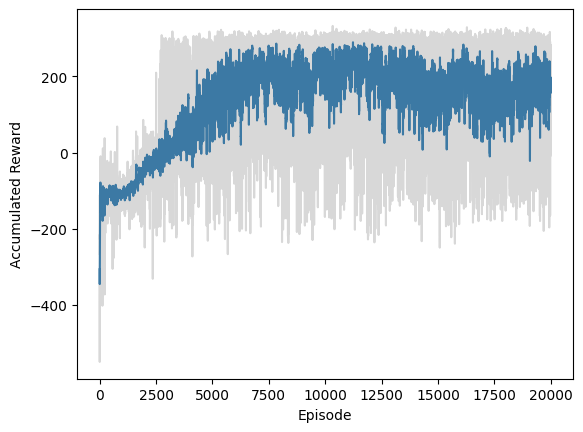
\includegraphics[width=0.8\textwidth]{Code/accumulated_reward.png}
    \caption{Accumulated reward over episodes.}
    \label{fig:accumulated_reward}
\end{figure}